\chapter{Testing}\label{chap:testing}

This chapter is dedicated to various testing techniques applied during implementation to improve the quality of the application in multiple dimensions.

\section{Automated testing}\label{sec:auto-testing}

% https://learn.microsoft.com/en-us/dotnet/core/testing/unit-testing-best-practices

Numerous \emph{unit} and \emph{integration} (without infrastructural dependencies) tests were written for both the frontend and backend to verify that individual modules and their assemblies meet functional requirements. Life containers were replaced by failing, stalling, or ordinary mocks.

Please note that \emph{end-to-end} tests were \underline{not} conducted, mainly because interactions among parts of the system involve straightforward scenarios. If necessary, frontend integration tests may be converted to end-to-end tests using the \emph{Playwright}\footnote{\href{https://playwright.dev/}{https://playwright.dev/}} framework or similar.

\subsection*{Frontend}

The frontend was tested with the Jest\footnote{\href{https://jestjs.io/}{https://jestjs.io/}} framework and React Testing Library\footnote{\href{https://testing-library.com/docs/react-testing-library/intro/}{https://testing-library.com/docs/react-testing-library/intro/}}. Test files reside in \texttt{\_\_tests\_\_/} folders close to the corresponding components and functions.

In total, \emph{676} tests were implemented, covering a range of tasks from simple rendering to simulating \emph{user actions}, such as advanced search, entity saving and removal, and navigation between panels. Test suites have the following structure:

\begin{minted}[fontsize=\footnotesize]{text}
// Component.test.tsx
describe("<Component />", () => {
  it("should allow users to search for routes", () => {
    const { getByRole, getByText } = render(...);
    fireEvent.click(getByRole("button", { name: "Search" }));
    expect(getByText("Found a total of")).toBeInTheDocument();
  });
  ... more tests follow ...
});
\end{minted}

The \texttt{describe} function forms a test suite. Test recipes are passed as lambdas in the parameters of \texttt{it} functions. The Jest test runner discovers them~automatically. HTML elements are accessed via \texttt{getByRole} and \texttt{getByText}. The \texttt{expect} function asserts whether a test condition is met. More primitives are used in the actual tests; however, their descriptions are omitted for brevity.

We estimate the test coverage to be between 60--80\%, depending on one's perception. Please note that this estimation is somewhat subjective. While writing tests, we focused on black-box testing, examining large chunks of code, as well as white-box testing, targeting individual components. Since tests were written for each component separately, adding new ones is straightforward.

Because we keep the state in Redux and Context~API containers, components that access them cannot be tested in isolation, and some sort of mocking is required. The \texttt{renderWithProviders} function helps to solve this issue by wrapping a component instance in standard providers. Then, rendering is customized via \texttt{props} and \texttt{options} parameters.

\begin{minted}[fontsize=\footnotesize]{text}
function render(props = getProps(), options = getOptions()) {
  return renderWithProviders(<Component {...props} />, options);
}
\end{minted}

Furthermore, the testing library recommends\footnote{\href{https://testing-library.com/docs/queries/about\#priority}{https://testing-library.com/docs/queries/about\#priority}} accessing elements of the DOM tree by roles and names. The frontend provides a reasonable level of \emph{accessibility} so that all tested elements can be reached and identified without referring to the \texttt{data-testid} attribute.

To execute tests, navigate to the \texttt{./app/frontend/} folder and type in:

\begin{minted}[fontsize=\footnotesize]{text}
$ npm run tests
\end{minted}

\subsection*{Backend}

Tests are located in projects whose names end with \texttt{.Test}. The MSTest\footnote{\href{https://github.com/microsoft/testfx}{https://github.com/microsoft/testfx}} test framework was our choice to describe and run individual test cases.

The layout of the backend is much simpler compared to the frontend; requests are processed by dedidated handlers in isolation. As a result, the number of~tests is only \emph{135}. We focused on modeling typical scenarios with malfunctioning in\-fras\-truc\-ture, individual handlers returning expected objects, and randomized tests for heuristics. By applying the \acs{dip} throughout the application, we were able to inject custom implementations of abstract interfaces defined by the \texttt{Core} into our tests. Test suites are expressed in the form of classes discoverable by the runner:

\begin{minted}[fontsize=\footnotesize]{text}
// ComponentTests.cs
[TestClass]
public class ComponentTests {
  [TestMethod]
  public void ShouldAssertNull() {
    Assert.IsNull(null);
  }
  ... more tests follow ...
}
\end{minted}

Similar to the previous section, we estimate the test coverage to a value between 50--70\%. Since each request invokes the corresponding pipeline that defines methods and functions to be called, overly detailed tests are unnecessary. The abil\-i\-ty of the backend to provide a valid response is partly covered by performance tests that check whether \acs{http} responses contain the status code~\texttt{200}.

To run tests, navigate to the \texttt{./app/backend/} folder and enter:

\begin{minted}[fontsize=\footnotesize]{text}
$ dotnet test
\end{minted}

\section{Performance testing}\label{sec:perf-testing}

The purpose of this testing phase is to justify that the system can meet~Requirements \ref{itm:q-response-time-places} and \ref{itm:q-response-time-routes}. Given that we have only one personal laptop, our~focus is solely on the \emph{response times} of individual requests rather than on the system's throughput.

The term ``reasonably large queries'' was mentioned in the requirements. We assume that only a minority of people are interested in casual walks longer than \emph{five} kilometers.

It is also specified that waiting 1~second for a place search and 2~seconds for a route search is deemed acceptable for the majority of users. This conclusion~is drawn from \cite{nielsen93}, where the author claims that a response time under 1~second ensures a user stays uninterrupted. Requests lasting between 1 and 10~seconds should indicate progress. Nonetheless, we should not overly restrict route search queries, as more time spent on calculations often leads to better results.

The parameters of the performance test environment are listed in Table~\ref{tab:performance-test-environment}. There are two more as\-sump\-tions we should state explicitly:

\begin{itemize}
\item responses were not rendered in a web browser,
\item and no network delay was included in the calculations.
\end{itemize}

The dataset for performance tests consisted of objects from the 10~largest cities of the Czech Republic, resulting in around $3 \times 10^{5}$ places and 817~keywords. It should be noted that the data are skewed; tourist cities often have a much higher number of places with no dependency on population.

Since we are interested only in a general trend, the results are presented in two types of graphs. The first type is a box-and-whisker diagram, whose interquartile range (IQR) is set to the distance between the lower quartile covering $25\%$ of the dataset, and the upper quartile covering $75\%$ of the dataset. The whiskers~extend up to $1.5 \times \text{IQR}$, and measurements outside of this range are considered outliers. The second type is a simple scatter plot.

\bgroup
\def\arraystretch{1.2}
\begin{table}[!ht]
\centering\footnotesize
\begin{tabular}{ l l }
\toprule
\textbf{Parameter}
  & \textbf{Value} \\
\midrule
Machine &
  Lenovo ThinkPad E580 \\
Processor
  & \makecell[l]{Intel(R) Core(TM) i5-8250U CPU @ 1.60GHz, \\ 1801 Mhz 4 Core(s), 8 Logical Processor(s)} \\
Primary memory
  & \makecell[l]{DDR4, 8GB, 2.40GHz} \\
Secondary memory
  & \makecell[l]{LENSE30256GMSP34MEAT3TA \\ PCIe NVMe SSD, 256GB} \\
Operating system
  & \makecell[l]{Microsoft Windows 11 Home, ver. 10.0.22621} \\
WSL version
  & 2.0.9.0 \\
Kernel version
  & 5.15.133.1 \\
\bottomrule
\end{tabular}
\caption{Parameters of the performance test environment.}
\label{tab:performance-test-environment}
\end{table}
\egroup

The source code for all performance tests is in the \texttt{./misc/perf/} folder, along with instructions on how to run them. The dataset is included in the electronic attachment for the thesis, as described in Attachment~\ref{sec:electronic-attachment}.

\newpage

Let us present the results of the tests, distinct for each \acs{http} endpoint.~Please note that the orange lines inside the boxes are \emph{medians}.

\vspace{1.5em}

\subsection*{GET /api/advice/keywords}

The input for this test consists of all keyword labels and the probability mass function determined by their frequencies. A trial randomly selects a keyword and then its prefix of length between 1 and 5. An \acs{api} call is issued for a fixed \texttt{\emph{count}} and this prefix.

Four different values of the \texttt{\emph{count}} parameter were considered, as shown along the $x$-axis of Figure~\ref{fig:perf-advice-keywords}. For each of them, 100~trials were performed.

These queries typically respond in $\leq 4~\text{ms}$. Outliers took at most $6~\text{ms}$.

\vspace{1.5em}

\subsection*{GET /api/entity/places/\{smartId\}}

In one trial of this test, a place identifier is randomly selected from all possibilities, and an \acs{api} call is made. The script performs 100~consecutive trials.

Figure~\ref{fig:perf-entity-places} illustrates that requests for retrieving places by \texttt{smartId} are about $1.5\times$ longer than those for keywords.

\vspace{6.0em}

\begin{figure}[!h]
  \begin{minipage}{0.48\textwidth}
    \centering
    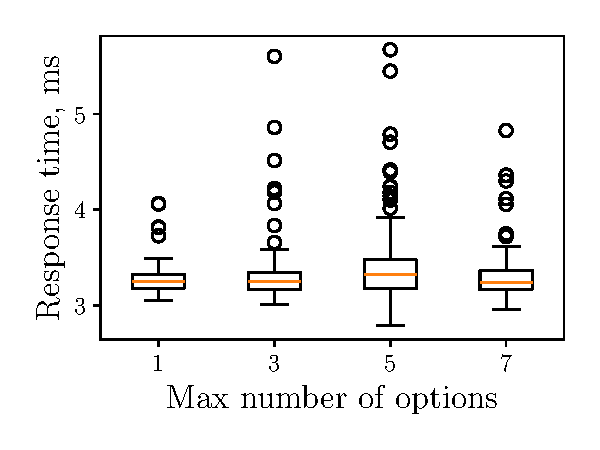
\includegraphics[width=\linewidth]{img/testing/perf-advice-keywords.pdf}
    \caption{Response times for fetching keywords by prefix.}
    \label{fig:perf-advice-keywords}
  \end{minipage}
  \hfill
  \begin{minipage}{0.48\textwidth}
    \centering
    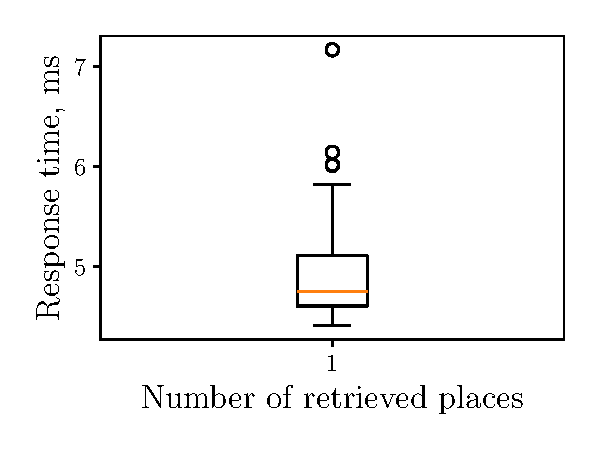
\includegraphics[width=\linewidth]{img/testing/perf-entity-places.pdf}
    \caption{Response times for retrieving places by \texttt{smartId}.}
    \label{fig:perf-entity-places}
  \end{minipage}
\end{figure}

\newpage

\subsection*{GET /api/search/direcs}

As part of the route search procedure, the \texttt{SearchRoutesHandler} class finds the shortest path connecting a sequence of places. Hence, direction search queries require a different approach because we are also interested in concrete numbers.

We want to test how the number of places visited by the shortest path and~its total length affect the response time of a request. The following pseudocode~cap\-tures the main ideas of the iterative testing procedure.

\begin{minted}[fontsize=\footnotesize]{text}
for count in [2, 3, 5, 7]:
  for city in 10 imported cities:
    for trial in [1, ..., 50]:
      locs <- SampleLocations(count, city)
      time, distance <- SearchDirecs(locs)
      result.append(count, time, distance)
\end{minted}

The graphs in Figure~\ref{fig:perf-search-direcs} illustrate the results. There is a strong tendency to complete a query in $\leq 30~\text{ms}$, even though distances may vary up to 200~km. The explanation for how \acs{osrm} achieves such performance is that it starts returning less detailed polygonal chains for very long paths.

\vspace{3.0em}

\begin{figure}[!h]
  \centering
  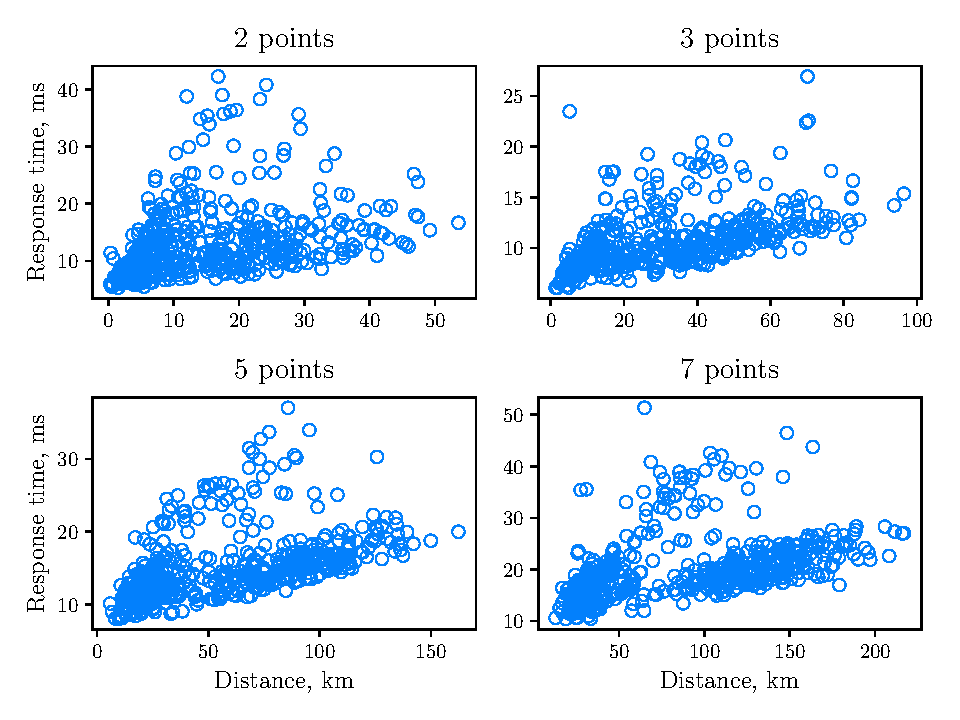
\includegraphics[width=\linewidth]{img/testing/perf-search-direcs.pdf}
  \caption{Response times for direction search queries.}
  \label{fig:perf-search-direcs}
\end{figure}

\clearpage

\subsection*{GET /api/search/places}

Place search requests were tested for various radii and different numbers of categories. Categories were represented by randomly selected keywords using a probability mass function similar to the first test; no attributes were configured.

When the number of categories is equal to $\infty$, the script sends an empty array instead of sampling, as specified in \ref{itm:f-search-places-cats}.

\begin{minted}[escapeinside=||,mathescape=true,fontsize=\footnotesize]{text}
for count in [1, 2, 3, |$\infty$|]:
  for radius in [1, 3, 5, 7, 10, 15]:
    for trial in [1, ..., 50]:
      center <- SampleLocation()
      categories <- SampleKeywordsWithPmf(count)
      time <- SearchPlaces(center, radius, categories)
      result.append(count, radius, time)
\end{minted}

Figure~\ref{fig:perf-search-places} confirms that radii up to 5~km are manageable within 1~s, but~larger values may result in longer request times.

We may find the current level of performance acceptable. However, clustering delegated to the server or a Web Worker becomes especially relevant for the ability of the system to provide a seamless user experience. Hence, this extension should be prioritized in later development.

\vspace{0.8em}

\begin{figure}[!h]
  \centering
  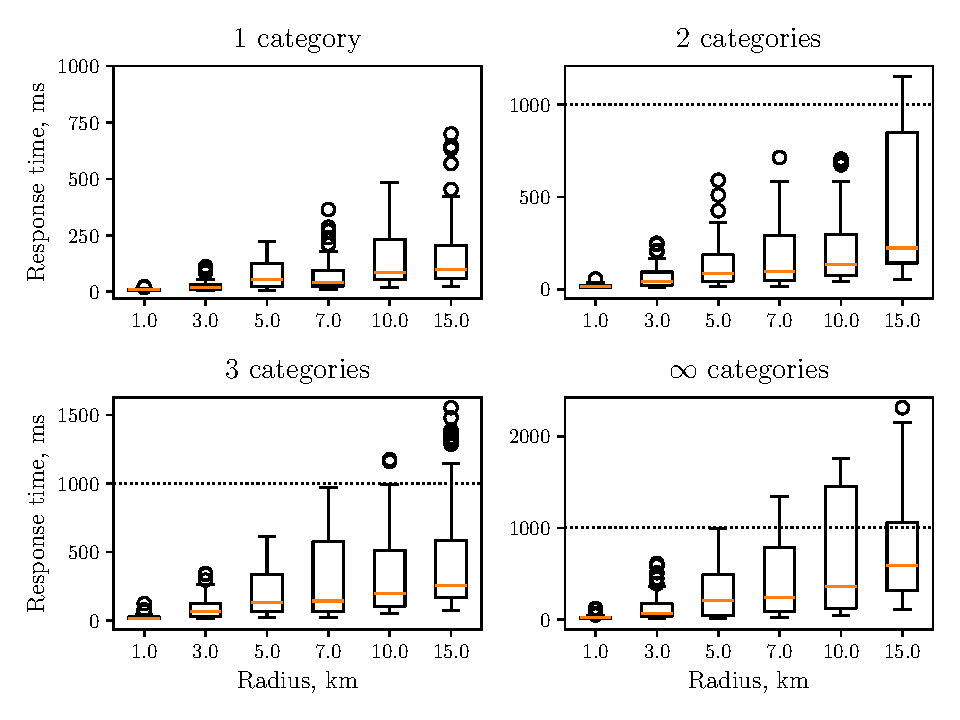
\includegraphics[width=\linewidth]{img/testing/perf-search-places.pdf}
  \caption{Response times for place search queries.}
  \label{fig:perf-search-places}
\end{figure}

\newpage

\subsection*{GET /api/search/routes}

This test has a structure similar to the previous one; please refer to the code snippet below for details. The \textbf{for}-cycle iterates over distances rather than radii. The source and target are set to the same location so that the generated routes are circular. The presence of arrows does not make a difference because the \acs{ifh} and \acs{ogh} have the same worst-case time complexity, $O(\lvert V \rvert \lvert C \rvert^{2})$.

\begin{minted}[fontsize=\footnotesize]{text}
for count in [1, 2, 3, 5]:
  for distance in [1, 3, 6, 10, 15, 30]:
    for trial in [1, ..., 50]:
      source <- SampleLocation()
      categories <- SampleKeywordsWithPmf(count)
      time <- SearchRoutes(source, distance, categories)
      result.append(count, distance, time)
\end{minted}

According to Figure~\ref{fig:perf-search-routes}, finding a route is a more computationally demanding task compared to the previous ones. For distances $\leq 6~\text{km}$, all requests were~answered in $\leq 2~\text{s}$. Rendering is not a problem either, as only one route at a time~is displayed on the map.

\vspace{3.1em}

\begin{figure}[!h]
  \centering
  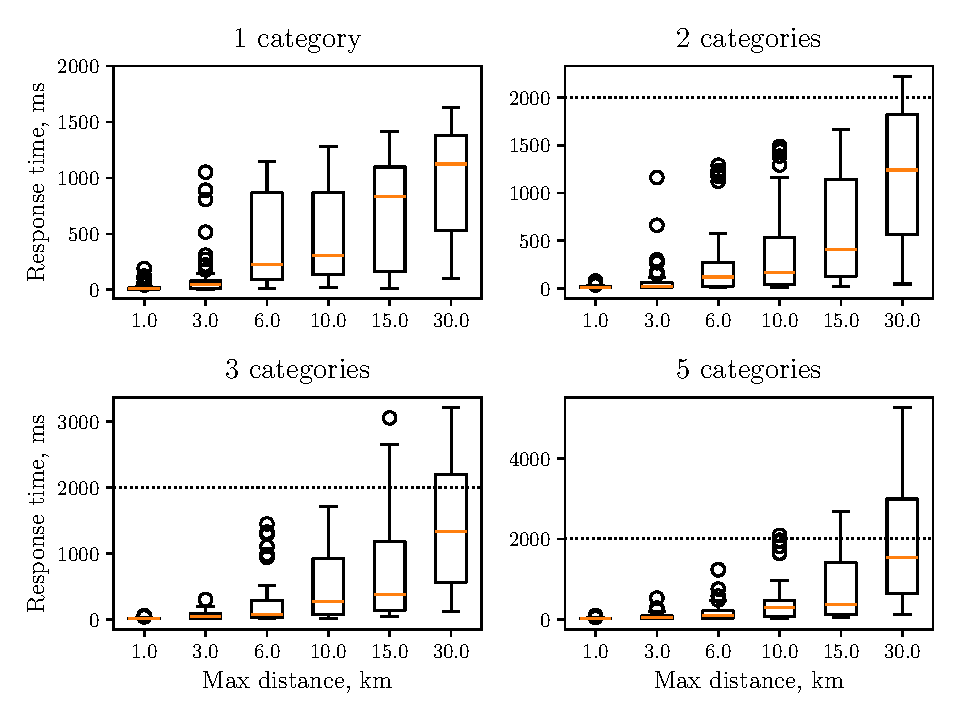
\includegraphics[width=\linewidth]{img/testing/perf-search-routes.pdf}
  \caption{Response times for route search queries.}
  \label{fig:perf-search-routes}
\end{figure}

\newpage

\section{Usability testing}\label{sec:user-testing}

% https://www.usability.gov/how-to-and-tools/methods/system-usability-scale.html

The usability of the user interface was measured using the \ac{sus} questionnaire, as proposed by Brooke~\cite{brooke96}. Respondents were asked to perform the following tasks in the given order on an attribute-rich dataset with places extracted from a bounding box around Prague\footnote{This dataset is not included in the electronic attachment due to license conditions. Please refer to \href{https://wiki.openstreetmap.org/wiki/Wikidata\#Importing\_data}{https://wiki.openstreetmap.org/wiki/Wikidata\#Importing\_data} for more information.}.

\begin{enumerate}
\item Find routes between two arbitrary points on the map with a distance at most 5~km that visits a castle and museum. Save any of the found routes.
\item Create a custom place, such as your favorite attraction, home, work, etc.
\item Find all restaurants with internet access and Italian cuisine around your favorite place. Navigate to the detailed view of any found restaurant and save it.
\item Find directions connecting your favorite place and the saved restaurant. Save any direction that appears in the result.
\item Delete the entities you have created.
\end{enumerate}

Before attempting to complete tasks, respondents were given a brief explana\-tion of the application's purpose without significant showcases. If they got stuck, we guided them by directing their attention to clues left in the test descriptions. Right after the tests, the respondents were asked to provide feedback by eval\-u\-at\-ing the statements from Attachment~\ref{sec:results-usability-testing}.

We successfully contacted four participants from diverse backgrounds. The first respondent was somewhat familiar with the concepts addressed in this thesis but had never independently accomplished any task. The second participant had a deep understanding of the theory behind algorithms and web development in general. The third respondent possessed practical experience in developing commercial web applications. Finally, the fourth respondent lacked specific knowledge or experience.

The results presented in Table~\ref{tab:results-usability-testing} indicate that the average \acs{sus} score for all participants is \textbf{85.00}. A score equal to 68 out of 100 is considered average, with higher scores indicating a more intuitive and usable application \cite{sauro11}.

Below, we state several valuable conclusions drawn from the survey evaluation and follow-up discussions.

\begin{enumerate}
\item The user interface was easy to learn but seemed cumbersome at first impression. Several participants expressed concerns about the structure of the dialog for adding a category as being too long or ill-aligned.
\item The conceptual difference between routes and directions was not immediately clear.
\item The test cases were not well-structured, particularly in the transition between the first and second steps. Also, starting with a test case other than searching for routes might be more effective.
\item The dialog for selecting a point might contain one more option that allows filtering based on address or arbitrary keywords, similar to \emph{\nameref{ssec:mapy-cz}}.
\item When searching for routes, the system checks if the starting point and destination are not too far from each other at the time of clicking the ``Search'' button. Some participants found it more convenient to be informed upfront.
\item In the results of a place search, sorting by the distance from the center point did not play a significant role. It was suggested to include a link to the corresponding detailed view and a ``Save'' button in each place's popup.
\item Some participants pointed out that three-dotted menu buttons should be considered to hide extra functionality, and separating the ``Save'' button might be beneficial. In contrast, other participants found the menu layout for managing results and favorite entities consistent.
\end{enumerate}

Despite all the efforts to create an intuitive user interface for accomplishing \ref{itm:g-ux}, there is still room for improvement. At the same time, the results showed that the application is easy to learn and get used to.
